\noindent
Con base en los principios expuestos en la Sección \ref{sec:ransac-teorico},
aplicamos una adaptación de RANSAC para estimar una homografía que haga coherente una retícula ideal con
las líneas de los cajones visibles en la imagen. Este enfoque conserva la robustez frente a outliers y
oclusiones propias del escenario de estacionamiento.

\begin{figure}[!ht]
    \centering
    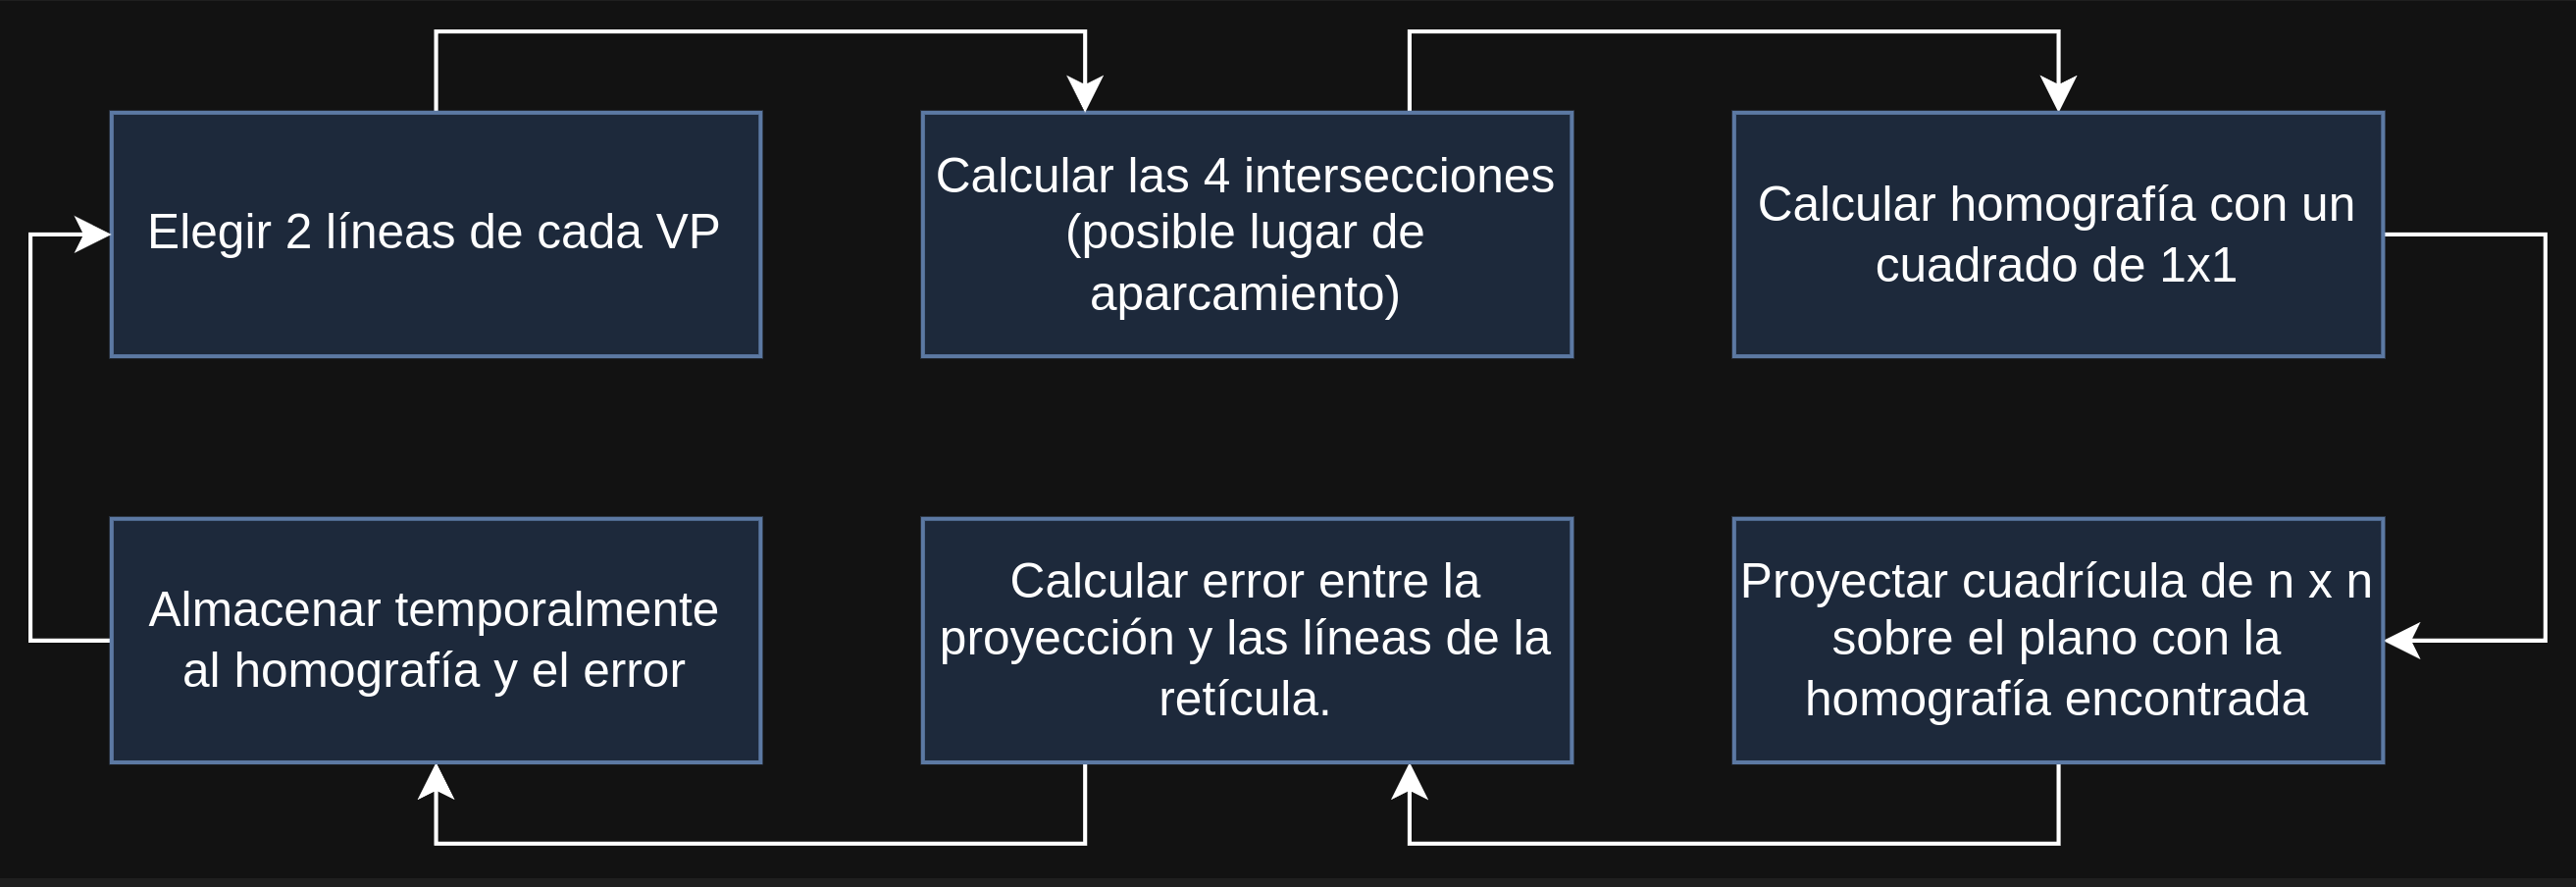
\includegraphics[width=0.95\textwidth]{img/3-metodo/ramsac_loop.png}
    \caption{Esquema del ciclo RANSAC propuesto para el ajuste de la retícula.}
    \label{fig:ramsac-flujo}
\end{figure}

\noindent
La variación propuesta sigue el ciclo de la Figura~\ref{fig:ramsac-flujo}:
\begin{enumerate}
    \item A partir de dos puntos de fuga estimados, agrupar las líneas detectadas en dos conjuntos según su punto de fuga asociado.
    \item Muestrear aleatoriamente dos líneas de cada conjunto y calcular las cuatro intersecciones \(P_1, P_2, P_3, P_4\) (producto cruzado de pares de rectas), que definen un candidato a cajón.
    \item Estimar la homografía \(\mathbf{H}\) que mapea el cuadrado canónico de lado 1 al cuadrilátero \(\{P_k\}_{k=1}^4\).
    \item Proyectar una retícula \(n\times n\) mediante \(\mathbf{H}\) sobre la imagen.
    \item Evaluar la consistencia entre la retícula proyectada y las líneas reales (por ejemplo, concordancia de orientación y proximidad en las regiones de soporte) y registrar una medida de ajuste.
    \item Almacenar temporalmente \(\mathbf{H}\) y su medida de ajuste; repetir desde el paso 2 durante \(N\) iteraciones.
\end{enumerate}

\noindent
Tras completar las iteraciones, se selecciona la homografía con mejor medida de consistencia 
como representación de la retícula en la imagen. 
Esta homografía permite extender el patrón más allá del campo visible, 
infiriendo la ubicación de cajones en puntos ciegos o parcialmente ocultos, 
lo que favorece la planificación de maniobras y el estacionamiento automático. 
Además, el esquema es robusto a líneas espurias y a oclusiones, 
y tiende a ser estable entre cuadros consecutivos al reutilizar la mejor homografía previa como
punto de partida (warm-start) . En la Figura~\ref{fig:ramsac-transform} se ilustra 
la transformación de un cuadrado canónico a un cajón detectado en la imagen mediante la homografía estimada.


\begin{figure}[!ht]
    \centering
    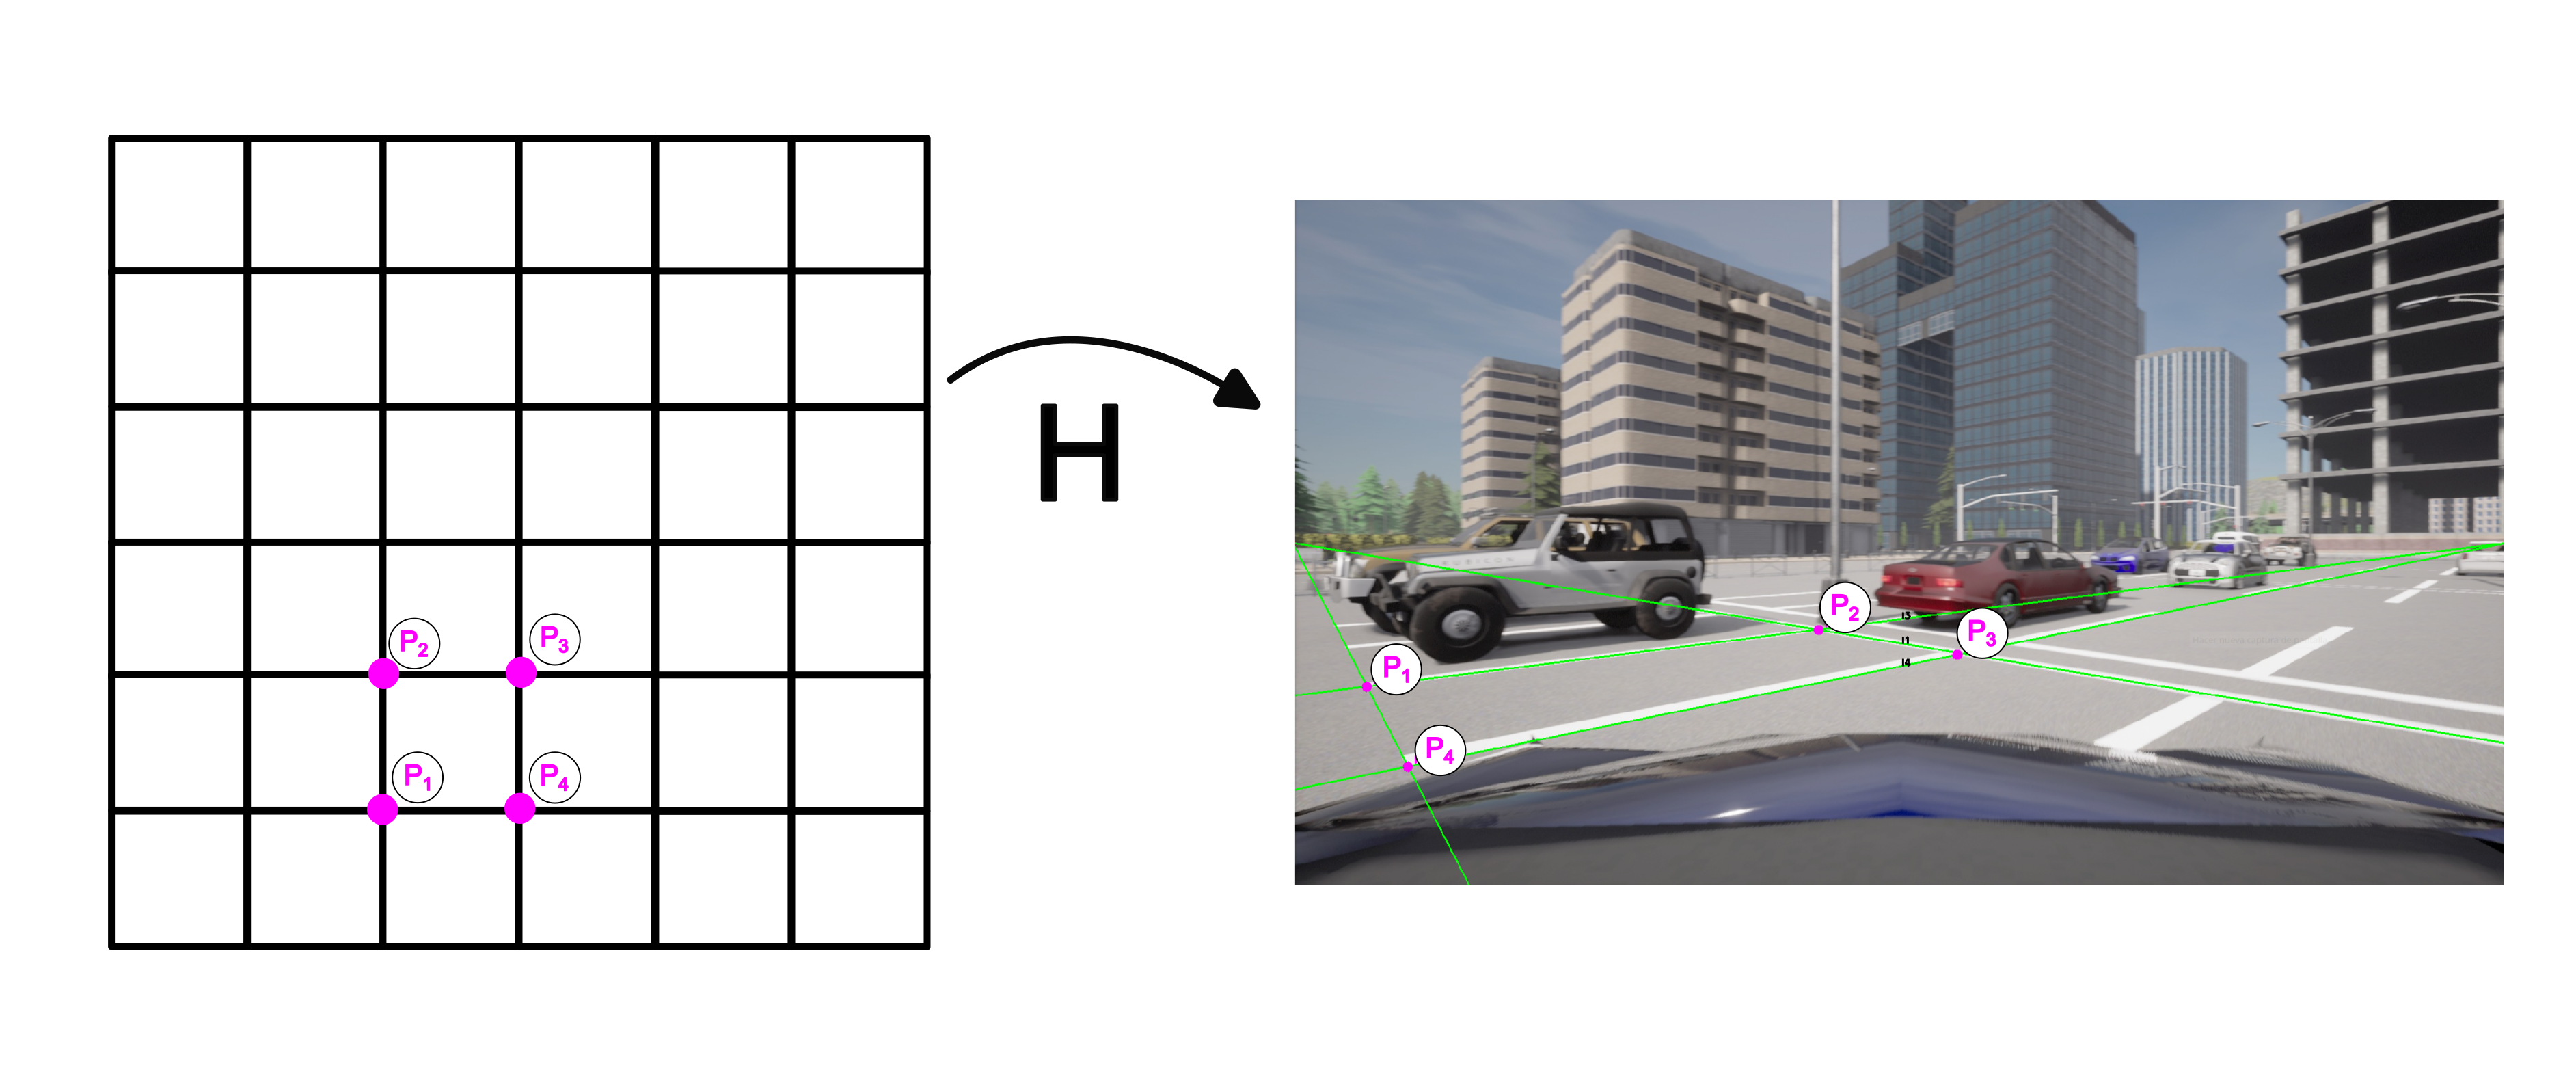
\includegraphics[width=0.95\textwidth]{img/3-metodo/transformacion.png}
    \caption{Estimación de una homografía \(\mathbf{H}\) que mapea un cuadrado canónico (izquierda) a un cuadrilátero de un cajón detectado en la imagen (derecha), permitiendo proyectar una retícula coherente aun cuando ciertas marcas no sean visibles.}
    \label{fig:ramsac-transform}
\end{figure}
